\documentclass{NSF}
\usepackage{hyperref}
\usepackage{units}
%\usepackage[small, bf]{caption}
\usepackage[numbers,sort&compress]{natbib}
\bibpunct{}{}{,}{s}{}{;}

\usepackage{color}
\usepackage{amssymb, amsmath}
%\usepackage{epstopdf}
\usepackage[final]{pdfpages}
%\usepackage{ulem}
\usepackage{verbatim}
\usepackage{amsfonts}
%\usepackage{subfloat}
%\usepackage{subfig}
%\usepackage{multirow}
\usepackage{authblk}
%\usepackage{array}
%\usepackage{footmisc}
%\usepackage{tabularx}
%\usepackage{sidecap}
\usepackage[noend]{algpseudocode}
\usepackage{algorithm}
\usepackage{setspace}
\usepackage{graphicx}
\usepackage[font={small}]{caption}
\usepackage{subcaption}
\usepackage[normalem]{ulem}
%\usepackage[margin=0.7in]{geometry}
\usepackage[usenames,dvipsnames,table,xcdraw]{xcolor}
\usepackage{rotating}
\renewcommand\Affilfont{\small}
\newcommand{\ignore}[1]{}
\newcommand{\ms}[1]{\textsc{#1}}
\graphicspath{{fig/}}

\usepackage[inline]{enumitem}

\newcommand{\doubleline}[2][c]{%
	\begin{tabular}[#1]{@{}c@{}}#2\end{tabular}}

\newtheorem{theorem}{Theorem}
%\newtheorem{acknowledgement}[theorem]{Acknowledgement}
%\newtheorem{algorithm}[theorem]{Algorithm}
% \newtheorem{axiom}[theorem]{Axiom}
%\newtheorem{case}[theorem]{Case}
%\newtheorem{claim}[theorem]{Claim}
%\newtheorem{conclusion}[theorem]{Conclusion}
%\newtheorem{condition}[theorem]{Condition}
%\newtheorem{conjecture}[theorem]{Conjecture}
%\newtheorem{corollary}[theorem]{Corollary}
%\newtheorem{criterion}[theorem]{Criterion}
%\newtheorem{definition}[theorem]{Definition}
%\newtheorem{example}[theorem]{Example}
%\newtheorem{exercise}[theorem]{Exercise}
\newtheorem{lemma}[theorem]{Lemma}
%\newtheorem{notation}[theorem]{Notation}
%\newtheorem{problem}[theorem]{Problem}
%\newtheorem{proposition}[theorem]{Proposition}
%\newtheorem{remark}[theorem]{Remark}
%\newtheorem{solution}[theorem]{Solution}
%\newtheorem{summary}[theorem]{Summary}
\newenvironment{proof}[1][Proof]{\textbf{#1.} }{\ \rule{0.5em}{0.5em}}

\usepackage{xargs} 
\usepackage[colorinlistoftodos,prependcaption,textsize=tiny]{todonotes}
\newcommandx{\note}[2][1=]{#1}


\newenvironment{packed_enum}{
\begin{enumerate}
  \setlength{\itemsep}{1pt}
  \setlength{\parskip}{0pt}
  \setlength{\parsep}{0pt}
}{\end{enumerate}}
\newenvironment{packed_itemize}{
\begin{itemize}
  \setlength{\itemsep}{1pt}
  \setlength{\parskip}{0pt}
  \setlength{\parsep}{0pt}
}{\end{itemize}}
\newenvironment{packed_desc}{
\begin{description}
  \setlength{\itemsep}{1pt}
  \setlength{\parskip}{0pt}
  \setlength{\parsep}{0pt}
}{\end{description}}

%%\def\glenn#1{{\textcolor{red}{GT note: #1}}}
\def\VB#1{{\textcolor{blue}{VB note: #1}}}
\def\SM#1{{\textcolor{orange}{#1}}}
\def\Shahab#1{{\textcolor{JungleGreen}{#1}}}


\def\figfmt{png}
\def\figsuffix{_reduced_size}
%\def\figsuffix{}
\def\MDDAF{\text{MDDAF}}
\def\DAF{\text{DAF}}

\def\dHAF{\text{-HAF}}
\def\HAF{\text{HAF}}
\def\HAFpeak{\text{HAF-peak}}
\def\HAFtrough{\text{HAF-trough}}
\def\HAFneutral{\text{HAF}_{\text{neutral}}}
\def\TMRCA{T_{\text{MRCA}}}

\def\all{\,\text{all}}
\def\car{\,\text{car}}
\def\ncar{\,\text{non}}

\def\MRCAall{\text{MRCA}^{\text{all}}}
\def\MRCAcar{\text{MRCA}^{\text{car}}}
\def\MRCAnon{\text{MRCA}^{\text{non}}}

\def\AlleleFreq{\text{AlleleFreq}}
\def\AlleleFreqNeutral{\text{AlleleFreq}_{\text{neutral}}}



\def\vecbold#1{{\bf#1}}
\def\mathbi#1{\textbf{\em #1}}

\def\Exp#1{\mathbb{E}\left[#1\right]} 

%\doublespacing % 2 line spacing
\onehalfspacing % 1.5 line spacing

\newcommand{\algoname}{\ensuremath{\text{PreCIOSS}}}
\def\skmer{\text{Skmer}}
\def\iSAFE{\text{iSAFE}}

%%%%%%%%%%%%
\makeatletter
\renewcommand\section{\@startsection {section}{1}{\z@}%                                                                                                         
                                   {-3.2ex \@plus -1ex \@minus -.2ex}%                                                                                        
                                   {2.0ex \@plus.2ex}%                                                                                                        
                                   {\normalfont\Large\bfseries}}
\renewcommand\subsection{\@startsection{subsection}{2}{\z@}%                                                                                                    
                                     {-2.95ex\@plus -1ex \@minus -.2ex}%                                                                                      
                                     {1.2ex \@plus .2ex}%                                                                                                     
                                     {\normalfont\large\bfseries}}
\renewcommand\subsubsection{\@startsection{subsubsection}{3}{\z@}%                                                                                              
                                     {-2.95ex\@plus -1ex \@minus -.2ex}%                                                                                      
                                     {1.2ex \@plus .2ex}%                                                                                                     
                                     {\normalfont\normalsize\bfseries}}
\renewcommand\paragraph{\@startsection{paragraph}{4}{\z@}%                                                                                                      
                                    {1.55ex \@plus1ex \@minus.2ex}%                                                                                           
                                    {-.7em}%                                                                                                                   
                                    {\normalfont\normalsize\bfseries}}
%%%%%%%%%%%%%%%%%%%%%%%%%%%%%%%%%%%%%%%%%%%%%%%%%%%%%%%%%%%%%%%%%%%%%%%%%
\DeclareMathOperator*{\argmax}{argmax}
\DeclareMathOperator*{\argmin}{argmin}
\DeclareMathOperator*{\trace}{trace}

% Siavash's supplementary
\newcommand{\beginsupplement}{%
  \setcounter{equation}{0}
  %\setcounter{theorem}{0}
  %\setcounter{lemma}{0}
  %\setcounter{corollary}{0}
  \setcounter{section}{0}
  \setcounter{figure}{0}
  \renewcommand{\theequation}{S\arabic{equation}}
  %\renewcommand{\thetheorem}{S\arabic{theorem}}
  \renewcommand{\thetable}{S\arabic{table}}%
  \renewcommand{\thefigure}{S\arabic{figure}}%
  \renewcommand{\thesection}{\Alph{section}.}%
  \renewcommand{\thesubsection}{S\arabic{section}.\arabic{subsection}}%   
  \clearpage
  \onecolumn
  \begin{center}
    \textbf{\huge Supplementary Material~\\~\newline}
  \end{center}
}

%% \usepackage{color}
%% \graphicspath{{figures/}}

\begin{document}

% A. Cover Sheet
% A number of the boxes contained on the Cover Sheet are
% electronically pre-filled as part of the FastLane login process
% Complete the rest of your info there

% B. Project Summary
\title{New algorithms for genome skimming and its applications}

\definecolor{grey}{rgb}{0.5, 0.5, 0.5}
\newcommand{\INST}[1]{{\color{grey} #1}}

\newsection{B}
\section*{Project Summary}


\paragraph{Intellectual Merit.} 
If successful, the proposed activities will allow the estimation of
genomic bio-diversity for a fraction of the current costs of labor and
genome sequencing. The proposal uses a number of innovative and novel
algorithmic and statistical techniques, and describes the first
systematic study of the feasibility of computing the genomic distance using only a small, random fraction of the genome.  If successful, the project will advance the field by providing a simple and inexpensive protocol for measuring biodiversity with higher sensitivity than is currently achievable. The investigators
have a strong history of prior research in related fields, but have
complementary expertise, in evolution and phylogenetic reconstruction
(Mirarab), and computational population genomics (Bafna).

\paragraph{Broader Impacts.}
Much of the planet's biodiversity is in the least developed and
poorest places on the planet. Rapid environmental change and
anthropogenic activities are degrading this bio-diversity and have
potentially severe and lasting impact on all people, including in the
U.S. The proposed tools enable the cataloging and measurement of
bio-diversity through inexpensive sequencing, and easy-to-adopt
laboratory protocols. While the proposal focuses on computational
tools, the experiments will demonstrate proof of concept and the
viability of larger sampling studies with a view towards deploying
them where they are most needed. The proposal will also help train
scientists who are better aware of the impact of rapid environmental
changes on ecology, and the role of genomics and computation in
investigating and alleviating these impacts. Through outreach activities, trainees will include undergraduate students from under-represented communities.

\paragraph{Keywords:} bioinformatics; computational genomics; computational evolution.


% C. Table of Contents 
% A Table of Contents is automatically generated for the proposal by FastLane

% D. Project Description
\clearpage
\newpage\newsection{D}
%\section*{Project Description}
\section{Introduction and Goals}
Anthropogenic pressure and other natural causes have resulted in
severe disruption of the global ecosystems in recent years, including
climate change with extreme weather events, change (loss) of
biodiversity, and invasion of non-native flora and fauna. The
deforestation of rainforests and degradation of natural habitats is
happening faster than efforts to study and understand the impact of
these environmental insults.  Beyond undesired changes, recent years
have also seen an increase in experimental genetics experiments that
could radically change the population distribution in an
environment. For example, the Target Malaria project is a \$75M effort
using CRISPR gene drives to genetically modify, and eliminate
mosquitoes (\emph{Anopheles}), and could be deployed in Africa within
2 years\cite{TargetMalaria}, but its impact on the local biogeography
is completely unknown.  Similar gene drives are being organized to
eliminate Avian malarial parasite carrying mosquitoes from
Hawaii\cite{Liao2017}, and Rodents from New Zealand\cite{Owens2017}.

The ability to quickly and inexpensively sample the taxonomic
diversity in an environment in real time is critical in this era of
rapid climate and biodiversity changes, and for the ethical conduct of
these directed evolution experiments in nature\cite{Oye2014}. Indeed,
such methods are specifically important for organisms such as
arthropods\cite{Beng2016} and small plants, which are among the most
abundant and diverse non-microbial organisms on Earth but lack
large-scale descriptions of biogeography and richness. However, large
cataloging surveys remain sparse. At least some of this discrepancy
can be attributed to the high cost of sorting and identifying samples
from large sampling collections.

%With the advent of next generation sequencing methods, 
The molecular technique of choice for measuring biodiversity is
(meta)barcoding\cite{Hebert2003,Savolainen2005,Taberlet2012}, which
involves DNA sequencing of taxonomically informative and
group-specific markers (e.g., mtDNA COI~\cite{Seifert2007,Hebert2003}
and 12S/16S \cite{Vences2005} for animals, plastid genes like trnl and
matK~\cite{Hollingsworth2009} for plants, and ITS~\cite{Schoch2012}
for fungi) that are variable enough for taxonomic identification, but
have flanking regions that are sufficiently conserved to allow for PCR
amplification using universal primers. Barcoding is used to
taxonomically identify species or in the case of meta-barcoding to
deconstruct the species composition of complex samples. Accurate
barcoding crucially depends on the coverage of the reference database
and the method used to search the database~\cite{Taberlet2012}.
Computational methods have been developed for finding the closest
match in a reference dataset of markers (e.g., TaxI\cite{taxl}), and
for placement of a query into existing marker
trees\cite{epa,pplacer}. The reference databases for these studies
consist of traditional barcode regions, such as COI in the Barcode of
Life Data System\cite{BOLD}.

The traditional barcoding pipeline has several drawbacks.  PCR for
marker gene amplification requires relatively high-quality DNA and
thus cannot be applied to samples in which the DNA is heavily
fragmented.  Moreover, since barcodes are short regions, their
phylogenetic signal is limited\cite{Hickerson2006b}.  For example, 896
of the 4,174 species of wasps could not be distinguished from other
species using COI barcodes\cite{Quicke2012}.  While low costs have
kept PCR-based pipelines attractive, falling costs of shotgun
sequencing have now made it possible to shotgun sequence 1-2Gb of a
reference specimen sample for $\le\$50$, inclusive of sample
preparation and labor costs.  Therefore, researchers have proposed
low-pass sequencing (\emph{genome-skimming}) as a viable approach to
barcoding\cite{Coissac2016}. These approaches identify
chloroplast/mtDNA marker genes in genomes by mapping to a reference
library or \emph{de novo} assembly\cite{Liu2013}.  Large databases
(e.g., through PhyloAlps~\cite{PhyloAlps} and NorBol~\cite{NorBol}
projects) are using genome-skimming to mine marker genes.  Our Danish
collaborators ({\bf letter: Gilbert}) have developed a similar
genome-skimming project, DNAmark~\cite{DNAmark}. However, they
realized that {\em accurate} assembly of organelle and marker regions
from genome-skims is non-trivial, and the approach discards the vast
majority of the reads and is thus wasteful.  Therefore, they posed an
interesting methodological question: \emph{can the unassembled data be
  used ``as-is'' for barcoding, saving on the labor-intensive task of
  mtDNA assembly and using all available genomic information?}

Motivated by this question, we consider the alternative approach where
low coverage genome-skims are used both to create the reference
library and the query dataset. We propose the development of
computational and statistical tools to address the following key
questions (Figure~\ref{fig:overview}):
\begin{packed_desc}
%[label={\bf A\arabic*}:]
\item [Aim 1:] 
\item [Aim 2:] 
\item [Aim 3:] 
\end{packed_desc}
\begin{figure}
\centering
  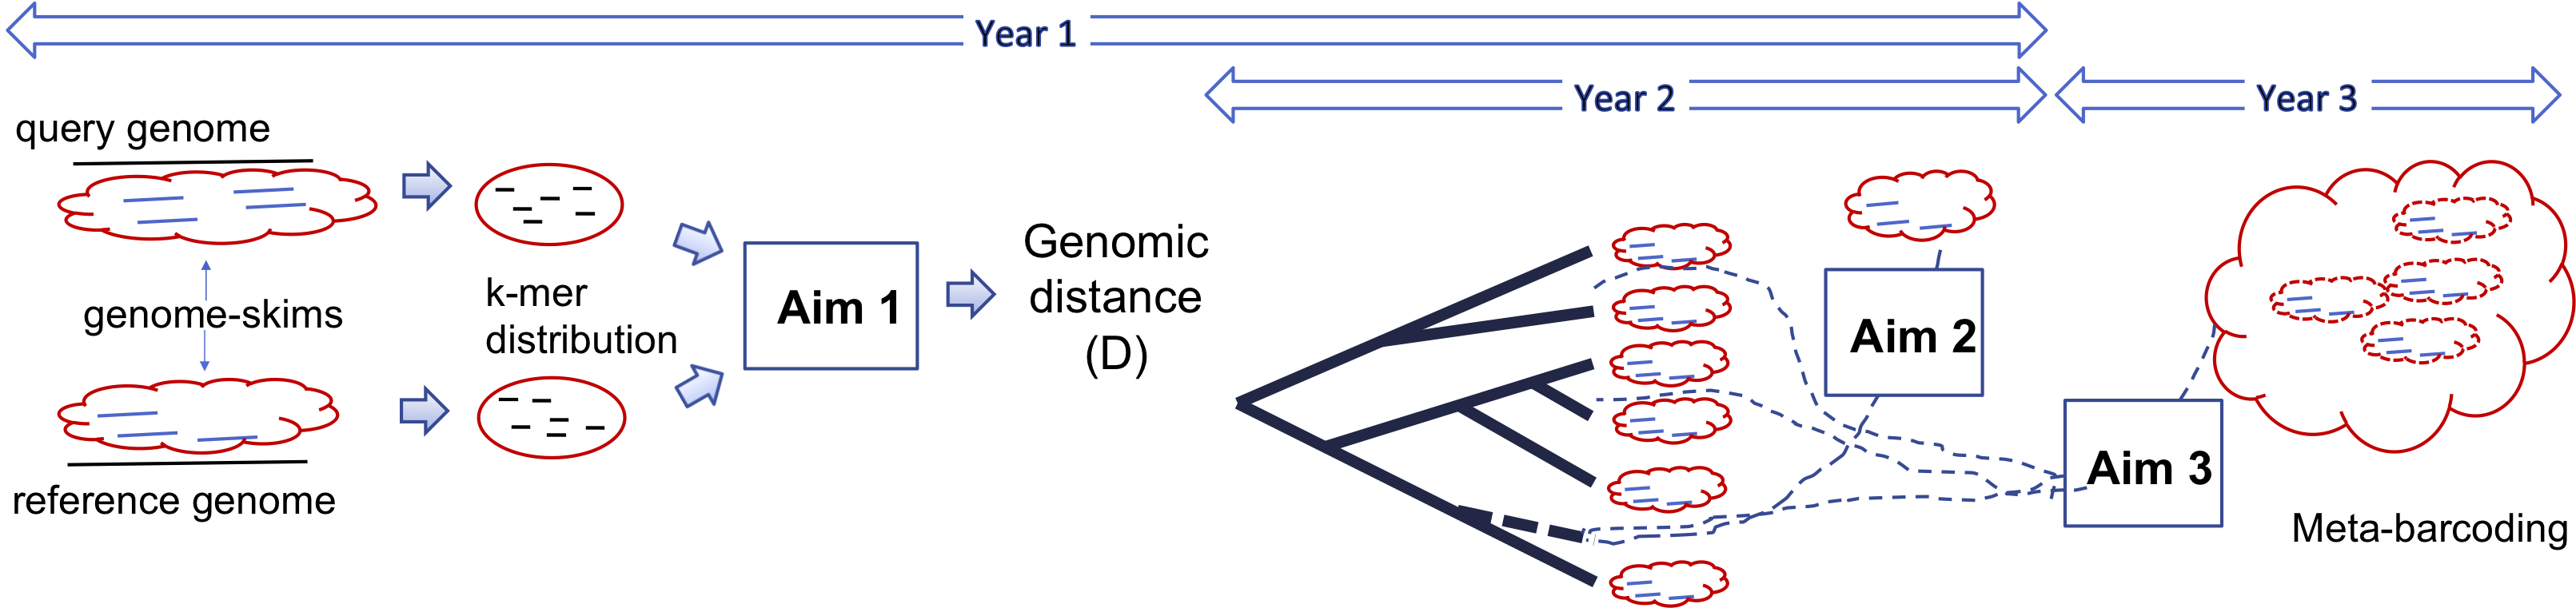
\includegraphics[width=1\textwidth]{fig/Overview.png}
\vspace{-20pt}\caption{{\bf Overview of the scientific aims.}}
  \label{fig:overview}
\end{figure}
As this is a \emph{short}, exploratory, proposal budgeting for four graduate student years, we will address Aims 1 (Year 1) and Aim 2 (Years 1 and 2) thoroughly and will perform exploratory empirical and theoretical work on Aim 3 (Year 3) in preparation for a larger, collaborative proposal.

\section{Broader Impacts}

The proposed activities have broad impact because some of the poorest and under-developed places have most of the
remaining bio-diversity in the world. The loss of this bio-diversity can
have severe and lasting impact on all people, including in the
U.S.A. However, even with dramatically falling costs, genomic
sequencing technologies have not penetrated these communities. We will use the grant period to reach out to scientists and build collaborations that start to catalog genome-skims, similar to
barcoding efforts such as the Consortium for the Barcode of Life.  
We will collaborate with Dr. Thomas Gilbert, leader of the center for GeoGenetics at the Natural History
Museum of Denmark on developing metabarcoding. 
We will also
initiate a collaboration with Dr. Ethan Bier (UC San Diego, and Tata
Institute of Genomics and society) who is developing CRISPR based
technologies to change \emph{Anopheles} population composition in some
locations in India with the goal of eliminating malaria. We will use
these initial studies to develop inexpensive protocols that will allow anyone in the world to gather genome-skims that can be
analyzed by our publicly available tools.  
Beyond these, 
we will make outreach efforts: i)
train STAR undergraduate students, recruited from both biology and CS;
ii) the annual Evolution meeting includes an outreach program promoting the understanding of computational technique; we will participate in Year 3 and use barcoding using genome-skims as an example  to promote computational understanding among biology undergraduates;
iv) we will hold local seminars to increase awareness of the impact of rapid environmental changes on
ecology and the role of 
computational genomics  in 
alleviating them.
%Taken together, the impact  of our proposed work exceeds the impact of the proposed algorithmic work.




\paragraph{Preliminary Results.}




\paragraph{{\large Challenges and proposed goals}.}


\paragraph{A1.3 Contamination.}
A major issue that we have so far ignored is 
the possibility that external DNA originating from parasites, diet, fungi, bacteria, and human contamination may be mixed 
with a supposedly single-species genome-skim.
The presence of such external DNA can negatively impact the estimated distance. 
%We plan to address this shortcoming in several ways.
%\begin{enumerate*}[itemjoin={.\quad},label=\roman*)]
%\item 
We will perform extensive tests
to quantify the robustness of \skmer\ to 
external DNA by manually injecting
fungal, bacterial, and human contamination.
Moreover, so far, we have tested \skmer\  only on simulated genome-skims. 
We plan to collaborate with our DNAmark colleagues
to test \skmer\ on real genome-skims from known species. 

To improve \skmer\ in the presence of external DNA,
several approaches can be considered.
For genome-skims in the reference library,
we can simply search a database using tools like BLAST~\cite{blast}, USearch\cite{usearch}, or Bowtie~\cite{Langmead2012a}, or faster k-mer based methods like Kraken~\cite{Kraken}  to find and eliminate bacterial or fungal contamination.
Note that the cost of preprocessing will be amortized over many searches.

For query sequences, even a fast classification tool like Kraken run
on all reads \textit{may} prove too slow.  But note that we don't need
identities of contaminants.  \emph{Given a query genome-skim, and a
  large `contaminant database' of genome skims from prokaryotes and
  fungi, we will develop super-fast algorithms for filtering
  contamination}.  We will test membership queries using Bloom filters
representing the union of k-mers in all contaminant
sequences. Consider a bit-vector $B$ of size $m$, where each of $n$
k-mers from a contaminant set is hashed using $h$ bits. Then, the
probability of a non-contaminant k-mer being hashed to $B$ by chance,
$p \le (1-e^{-\frac{hn}{m}})^h$. We will denote a read as a
contaminant if a fraction $\theta$ of its k-mers are hashed to
$B$. For small $p$, the probability of mis-classifying a read as a
contaminant is bounded using Chernoff's bound to be
$\le\text{exp}(-\ell(\theta-p)^2)$.  Adjusting $\theta$, we can also
detect contamination from species {\em close to} but not identical to
those in our database.  Thus, Bloom filter may provide a super-fast
way of eliminating all contaminant reads.

For even higher speeds, {\em we will develop algorithmic strategies to
  compute the true distance without eliminating contaminants}.  For a
query genome-skim with a mix of $k$-mers from the real species ($A$)
and those from contaminants ($C$), and reference skim $B$, let $J'$ be
the Jaccard computed without filtering.  We can estimate the fraction
of contamination $w=\frac{|A|}{|A\cup C|}\approx\frac{|A|}{|A|+|C|}$
by running Kraken or the Bloom filter on a small subset of reads.  We
expect contaminants to have very low similarity to the main query
species (e.g., fungal DNA in an insect query). Thus, their
contribution to the shared $k$-mer set is negligible (i.e., $|A\cap
C|\approx |B\cap C|\approx 0$).  Note also that $|A\cup B \cup C|$ and
$|A\cup C|$ can be easily computed using JellyFish.  Then, we can
derive the corrected $J$:
\vspace{-6pt}
\begin{small}
$$J=\frac{|A\cap B|}{|A\cup B|}=\frac{|A\cap B|/{|A\cup B \cup C|}}{|A\cup B|/|A\cup B \cup C|}=\frac{J'}{1-\frac{|C|}{|A\cup B \cup C|}}=\frac{J'}{1-(1-w)\frac{|A\cup C|}{|A\cup B \cup C|}}\; .
\vspace{-3pt}
$$
\end{small}
Thus, we can use Equation~\ref{eqn:distance_estimate_penalized} with
this contamination-corrected estimate of $J$.  This way of handling
contamination is essentially a simpler case of meta-barcoding (Aim 3)
because we assume {\em a priori} that contaminants are distant from
the main query species and do not seek their identity.

\vspace{-5pt}
\section{Intellectual merit}
\vspace{-5pt}
The proposed research creates a novel paradigm for measuring
biodiversity. If successful, the activities will allow us to sample
genomes of multiple organisms for a fraction of the current costs of
labor and genome sequencing required for other approaches. The
proposal uses a number of novel algorithmic and statistical ideas to
correctly estimate genomic distance based on
genome-skims. Specifically, it will be the first systematic analysis
of how close we can get to computing the genomic distance using only a
small and random fraction of an individual's genome. The proposed
methods can easily be extended to other vexing problems such as the
identification of phylogenetic placement of a previously unknown
organism, provenance of a museum animal, 
sibling analyses, and possibly forensic
science. The investigators have a strong history of prior research in
related fields, but have complementary expertise. Lead PI Mirarab is
an expert in evolution and phylogeny reconstruction of organisms and
helped reconstruct the state of the art in avian\cite{avian} and plant~\cite{1kp-pilot}
phylogeny, has developed highly
used tools for phylogeny inference~\cite{astral,astral2} and
metagenomics\cite{sepp,tipp}. PI
Bafna has expertise in genomics, and the use of novel techniques for
analyzing complex structural variation\cite{Turner2017} as well as the
development of new sequencing technologies and computational tools for
analyzing the resulting data\cite{Chu2017,Edge2017,Patel2014}. He also has expertise in
population genetics, and the impact of environment (selection
processes) in shaping the population genetic variation landscape\cite{Ronen2014,Ronen2015}.



%\section{Broader Impacts of the Proposed Work}


\vspace{-5pt}
\section{Results from Prior NSF Support}
\vspace{-5pt}

\noindent
\emph{\underline{Bafna}}: NSF-III (1318386) ``Algorithms for decoding complex patterns of genomic variation'' (\$500K, 9/01/13-8/31/17).  
{\bf Intellectual Merit:} Multiple publications resulted from this grant\cite{Lo2013,Ronen2013,Zhou2013,Lo2013b,Patel2014,Udpa2014,Kramer2014,Kinsella2014,Ronen2014,
Chen2015,
Zakov2015,Ronen2015,Flannery2015,Beyter2016,Patel2016,Stobdan2015,
Azad2016, Ronen2016, Edge2017, Iranmehr2017, Azad2017, Stobdan2017}, focused on exploiting the allele frequency spectrum for identifying regions under selection, experimental evolution, haplotype assembly, and decoding of complex structural variation. {\bf Broader Impacts:} include software tools, CLEAR for analyzing experimental evolution\cite{Iranmehr2017}, InPhaDel\cite{Patel2016} and Hapcut2\cite{Edge2017} for haplotyping, and PreCIOSS for identifying carriers of a selective sweep\cite{Ronen2015}.

\noindent
\emph{\underline{Mirarab}}: III (1565862) ``Using Genomic Context to Understand Evolutionary Histories of Individual Genes'' (\$175,000, 7/1/2016--6/30/2018). {\bf Intellectual Merit:} 
Several publications have results from the grant~\cite{distique,MVroot,Shekhar2017,insects,astral3,Mai2017,dual-birth}.
{\bf Broader Impacts:} 
include several publicly available software
tools: DISTIQUE~\cite{distique},
MV Rooting~\cite{MVroot}, ASTRAL-3~\cite{astral3}, and TreeShrink~\cite{Mai2017}.
All tools are available at
{\tt http://eceweb.ucsd.edu/~smirarab/software.html}.
%   \url{https://github.com/smirarab/},
%   \url{https://github.com/uym2/},
%     \url{https://github.com/uym2/}, and
%     \url{https://github.com/niemasd}.
%   \url{https://github.com/smirarab/ASTRAL},
%   \url{https://github.com/uym2/MinVar-Rooting},
%   \url{https://github.com/uym2/TreeShrink},
%     \url{https://github.com/esayyari/DISTIQUE},
%   \url{https://github.com/niemasd/Dual-Birth-Model}
We have also created benchmark datasets
for the community to use:
%   \url{https://uym2.github.io/MinVar-Rooting/},
%   \url{https://esayyari.github.io/InsectsData},
 {\tt https://sites.google.com/eng.ucsd.edu/datasets/}.
 We also mentored three undergraduate students, one through the STAR program, through this project.


% E. References Cited
\newpage\newsection{E}
\renewcommand\refname{References Cited}
\bibliography{refs,smmendeley,siavashmendeley,shahab,vb}
% I prefer to use the IEEE bibliography style. 
% That's  NOT required by the NSF guidelines. 
% Feel Free to use whatever style you prefer
\bibliographystyle{ieeetr}
%\bibliographystyle{IEEEtran}

% F. Biographical Sketch(es)
\newpage\newsection{F}
%\renewcommand\refname{Biographical Sketches}
\section{Biographical Sketches}
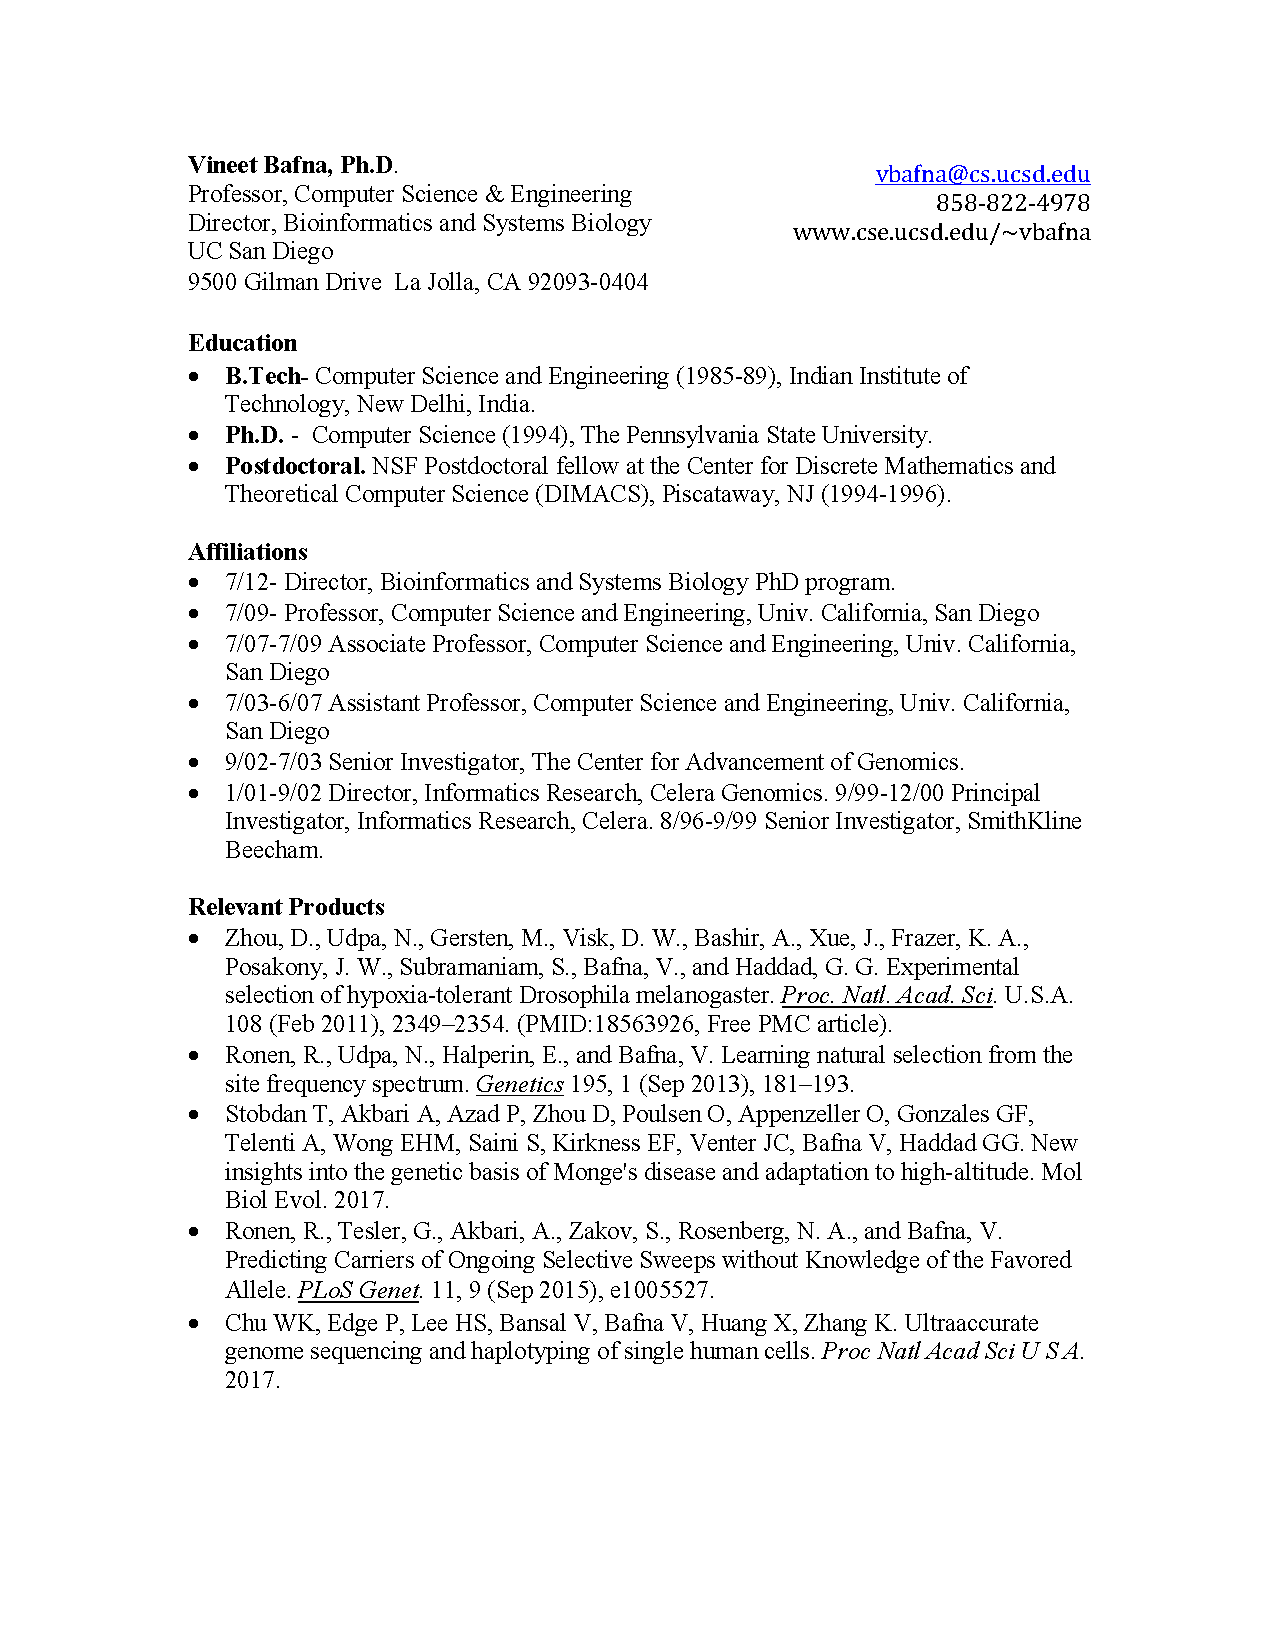
\includepdf[pages=-]{sections/pdfdocuments/VineetBafnaNSF.pdf}



% G. Budget Justification
\newpage\newsection{G}
\section{Budget Justification}
% No more than 3 pages!!! 
\subsection{A. Senior Personnel}
\noindent{\bf A1.} Includes PI at 10\% CY.
\subsection{B. Other Personnel}
\noindent{\bf B3.} Includes stipend for one graduate student for each calendar year of the project.  
\subsection{C. Fringe Benefits}
Fringe benefits are calculated at a rate of X\% for faculty, Y\% for graduate students.  
\subsection{E. Travel}
1) all travel (both domestic and foreign) must now be justified. 
2) temporary dependent care costs above and beyond regular dependent care that directly result from travel to conferences are allowable costs provided that the conditions established in 2 CFR § 200.474 are met.
\subsection{G. Other Direct Costs}
1) Includes coverage on costs of computing devices
2) The charging of computing devices as a direct cost is allowable for devices that are essential and allocable, but not solely dedicated, to the performance of the NSF award
\noindent{\bf G5.} Includes tuition for graduate students participating in the program.
\subsection{H. Indirect Costs}
Overhead at a rate of X\% is charged on all direct salaries and wages, applicable fringe benefits, materials and supplies, services, travel and subawards up to the first \$X of each subaward. Excluded are equipment and the portion of each subaward in excess of \$X.


%  H. Current and Pending Support
\newpage\newsection{H}
\section{Current \& Pending Support}
%% \begin{tabular}{ll}
%% \textbf{Investigator:} 			& \\
%% \textbf{Project Title:}			& Put your Proposal title here\\
%% \textbf{Project Location:}		& \\
%% \textbf{Source of Support:} 	& NSF\\
%% \textbf{Total Award Amount:} 	& \\
%% \textbf{Total Award Period:}	& \\
%% \textbf{Status:}				& Pending (this project) \\
%% \end{tabular}
%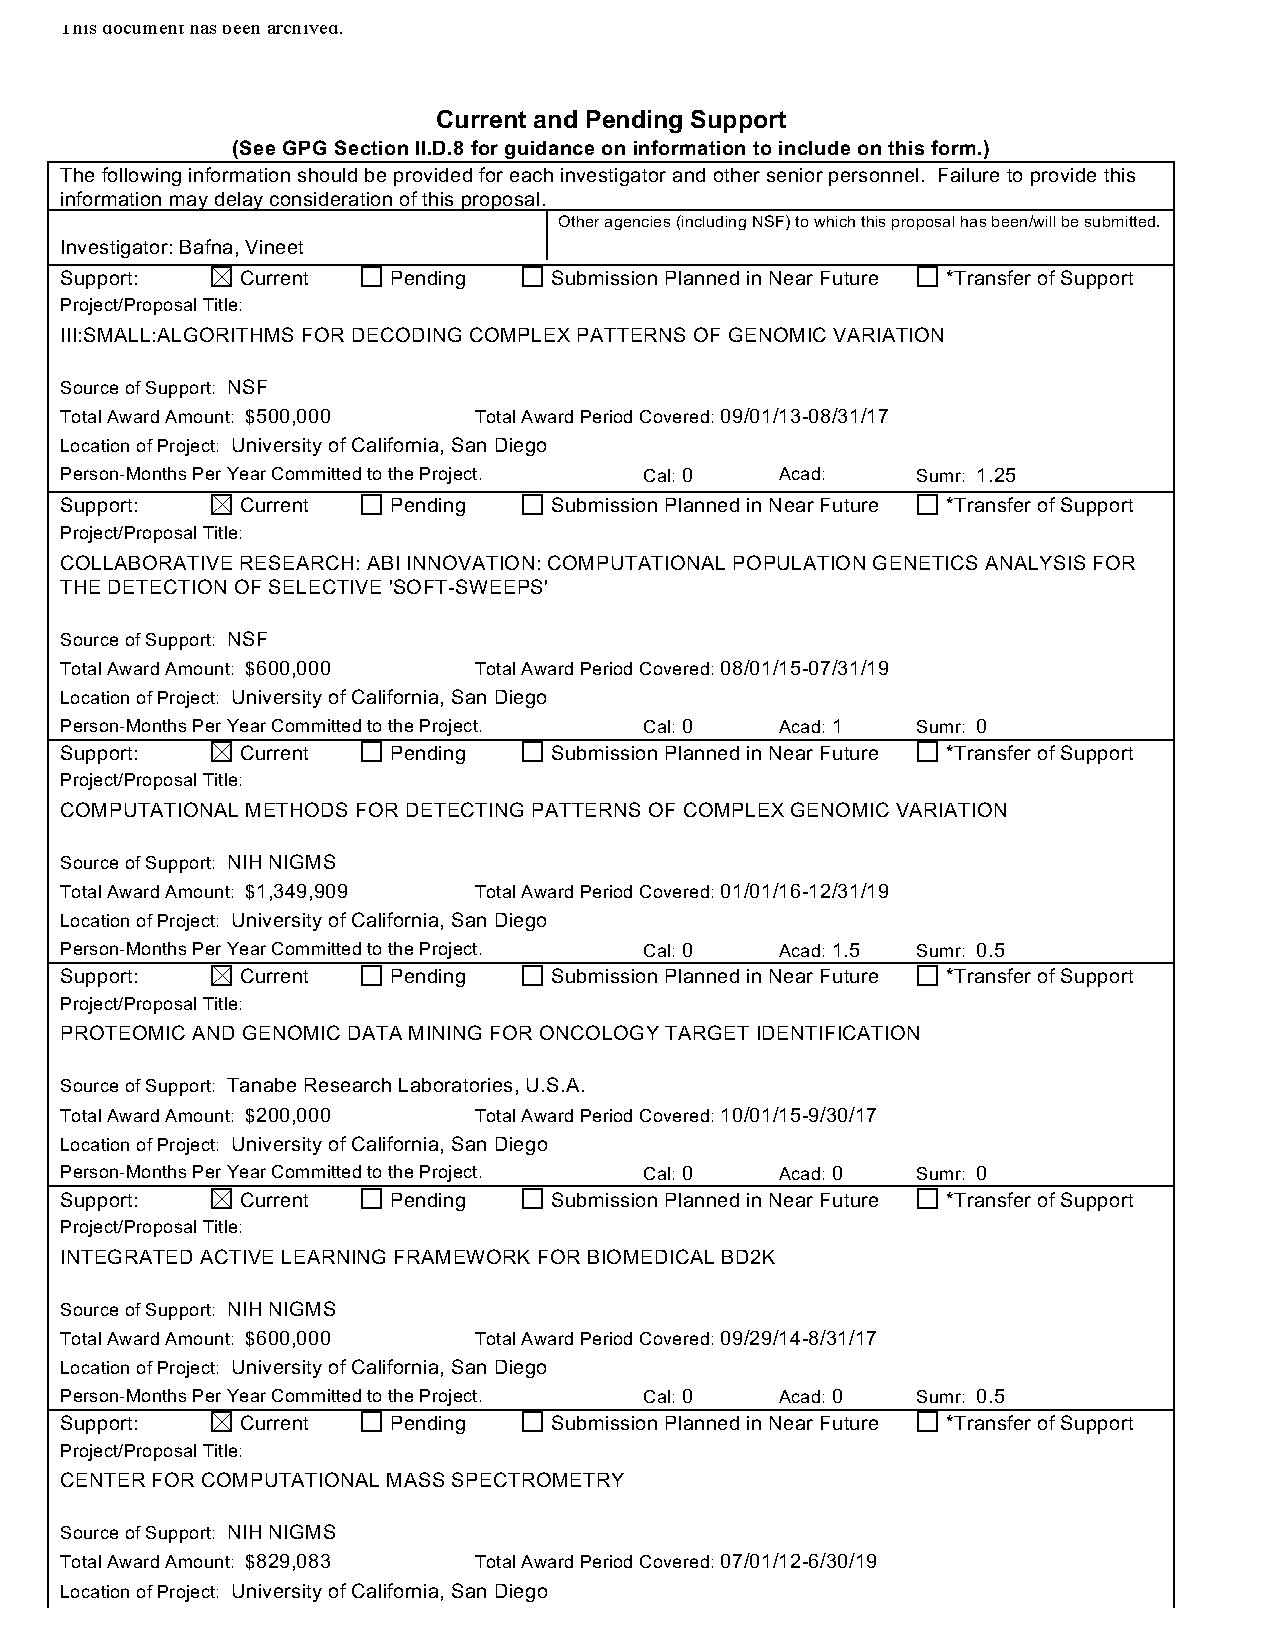
\includepdf[pages=-]{sections/pdfdocuments/BafnaCP.pdf}


% I. Facilities, Equipment and Other Resources
\newpage\newsection{I}
\section*{Facilities, Equipments, \& other Resources}

\paragraph{Collaborations:}




\subsection*{Facilities}

The Bafna Lab is in the UC San Diego Computer Science and Engineering (CSE) Department, located within the Computer Sciences building, a 135,000 sq. ft. high technology facility within the Jacob School of Engineering campus. Vineet Bafna's Bioinformatics laboratory encompasses approximately 1600 sq. ft. of dry lab space within the CSE building, and is adjacent to other labs focusing also on bioinformatics. There are 4 rooms, each about 40x10 sq feet, containing interactive 6x6 ft. cubicles, space for interacting and resting, with enough space for about 30 researchers. 
Irwin Jacobs, the founder of Qualcomm, has longstanding relations with our department, having been a professor at UCSD for many years. UCSD’s CSE Department embodies the University's tradition of excellence as a world-class leader in computer science and engineering education and research. CSE is in a period of exciting growth and opportunity. Ranked in handful of top programs in the country, the CSE is dedicated to research, education and overall excellence. The Bioinformatics Group within CSE has a focus on Genomics/Genetics, studying problems relating to genome rearrangements, structural variation, deep-sequencing, and population genetics, with a focus on novel analyses of data from high throughput technologies including sequencing, genotyping and mass-spectrometry. CSE Bioinformatics is an integral part of a vibrant Bioinformatics PhD program on campus with faculty from Biochemistry, Bioengineering, Biology, Mathematics, Medicine, Pharmacy, and Cancer Biology. 

The Mirarab lab is located in the Electrical and Computer Engineering (ECE) department of UC San Diego located at Jacobs Hall. It's a large dry lab that hosts eight graduate students. PI Mirarab has an office in the same building.

\subsection*{Equipment}

The proposed work requires computational platforms for studying the performance of the methods that will be developed. 
Both PIs  have access to a variety of computational resources to conduct the work, as described below. 

\paragraph{SDSC}
We are linked with the rest of campus via a 10 Gb/sec fiberoptic network, which provides access to the San Diego Supercomputer Center (SDSC), a unique national facility, with a variety of vector, multithreaded, and parallel supercomputers as well as a state-of-the-art high-performance visualization tools.
PI Mirarab currently has close to 1,000,000 hours of allocations on the SDSC cluster through NSF's XSEDE initiative. 
PI Mirarab will write renewal XSEDE proposals
for continuing his work on phylogenetics.
If this proposal is granted, 
we will request further allocations from XSEDE for conducting this project and analyzing real biological datasets that would accompany this project. 

\paragraph{TSCC.} 
PI Mirarab has access to the Triton Shared Computing Cluster (TSCC) cluster (\url{http://idi.ucsd.edu/computing/}) at San Diego Computing Center (SDSC). The PI has purchased an equivalent of 1.6 million cpu hours on the cluster that will last for the next two years, and the structure of TSCC will enable his lab to use at least those many hours of computing time. More specifically, the PI has purchased two nodes, each with 24 cores (Intel Xeon processor @ 2.5GHz) and 128GB of memory. The cluster is maintained by SDSC, with subsidized maintenance costs, and access to extra computational resources when the work load permits.

\paragraph{Mirarab's big data cluster.}
PI Mirarab has created a cluster of 70 server nodes, each with an Intel(R) Xeon(R) CPU iwth 7 cores. The members of the lab have full access to this cluster, which the PI shares with 4 other faculty in the ECE department. 


\paragraph{Vineet Bafna's Bioinformatics laboratory.}%encompasses approximately 1600 sq. ft. of dry lab space within the CSE building, and is adjacent to other labs focusing also on bioinformatics. There are 4 rooms, each about 40x10 sq feet, containing interactive 6x6 ft. cubicles, space for interacting and resting, with enough space for about 30 researchers.
Each cubicle contains a customized computer terminal, running an Intel Core i7 processor (with 8 processing threads @ 3Ghz), with 16 GB RAM and 2 TB of storage per computer. The Lab also has a Central Computer Linux Cluster, with 5 nodes, each with 24 cores and 128 GB RAM, and 128 TB storage space in total for data-intensive projects. 


\subsubsection*{Other}

All of the members of the both Mirarab and Bafna lab are proficient in the following computer languages: C++ (used to generate data filtering pipelines), PERL (used to interact with online databases), Python, Java, as well as Matlab and R for statistical analysis. Each person is familiar with algorithm development, data structure classes. 
Almost all of the proposed research uses free software, but additionally, PIs have access to simulation tools such as MATLAB and SIMULINK, if needed. 




% J. Special Information and Supplementary Documentation
\newpage\newsection{J}
\subsection*{Data Management Plan}

The Intellectual property and data generated under this project will
be administered in accordance with both University (\url{http://invent.ucsd.edu/invent/us/mission/policies-procedures/}) and NSF policies,
including the NSF Data Sharing Policy. Immediately after the grant is
funded, we will create a server as the single point of access for all
artifacts generated from the project.
\begin{packed_enum}
\item 
\item 
\end{packed_enum}




		% Data Management Plan (Required)
%\input{sections/postdoc} % Postdoctoral Researcher Mentoring Plan (if applicable)

\end{document}
